\section{Progettazione logica}
\subsection{Stima del volume dei dati}
Si suppone che siano state giocate 10 partite alla quale hanno partecipato ogni volta 4 giocatori diversi. Le partite prevedono mediamente 70 tessere in totale e 8 seguaci per ogni giocatore.
\medskip

\centerline{\begin{tabular}{ |l|c|c| }
\hline
\textbf{Concetto} & \textbf{Tipo} & \textbf{Volume} \\
\hline
Player & E & 40 \\
Participation & R & 40 \\
PlayerInGame & E & 40 \\
Having & R & 40 \\
Color & E & 10 \\
\hline
Meeple & E & 320 \\
Owning & R & 320 \\
Classification & R & 320 \\
BasicMeeple & E & 1 \\
ExpansionMeeple & E & 1 \\
Using & R & 1 \\
\hline
Gameset & E & 1.500 \\
Classification & R & 1.500 \\
BasicGameset & E & 5 \\
ExpansionGameset & E & 0 \\
Using & R & 0 \\
\hline
Game & E & 10 \\
Participation & R & 40 \\
Hosting & R & 10 \\
Using & R & 10 \\
\hline
Expansion & E & 4 \\
\hline
Server & E & 10 \\
Location & R & 10 \\
Region & E & 6 \\
Placement & R & 6 \\
Continent & E & 4 \\
Specifically & R & 6 \\
CardinalPoint & E & 5 \\
\hline
\end{tabular}
\begin{tabular}{ |l|c|c| }
\hline
\textbf{Concetto} & \textbf{Tipo} & \textbf{Volume} \\
\hline
Tile & E & 700 \\
Composition & R & 700 \\
Classification & R & 700 \\
BasicTile & E & 18 \\
ExpansionTile & E & 7 \\
Using & R & 7 \\
\hline
TileSection & E & 9.100 \\
Subdivision & R & 9.100 \\
Location & R & 9.100 \\
Classification & R & 9.100 \\
Placement & R & 200 \\
TileSectionType & E & 13 \\
Preceding & R & 12 \\
\hline
TileTypeConfiguration & E & 325 \\
Description & R & 325 \\
Regarding & R & 325 \\
Composition & R & 325 \\
\hline
\end{tabular}}

\subsection{Descrizione delle operazioni principali e stima della frequenza}
Si suppone che ogni giorno vengano giocate 10 partite alla quale partecipano ogni volta 4 giocatori diversi. Le partite vengono sempre concluse nell'arco della giornata e si prevede che mediamente vengono giocate 70 tessere a partite.
\medskip

\centerline{\begin{tabular}{ |c|l|c| }
\hline
\textbf{Cod.} & \textbf{Operazione} & \textbf{Frequenza} \\
\hline
1 & Creare una nuova partita & 10 al giorno \\
\hline
2 & Visualizzare i server di gioco disponibili & 10 al giorno \\
\hline
3 & Visualizzare tutte le espansioni & 10 al giorno \\
\hline
4 & Creare un nuovo giocatore & 40 al giorno \\
\hline
5 & Visualizzare tutti i colori & 40 al giorno \\
\hline
6 & Visualizzare il giocatore corrente & 700 al giorno \\
\hline
7 & Visualizzare la tessera corrente & 700 al giorno \\
\hline
8 & Ruotare la tessera corrente & 300 al giorno \\
\hline
9 & Piazzare la tessera corrente & 700 al giorno \\
\hline
10 & Piazzare o rimuovere un seguace su una sezione di una tessera & 300 al giorno \\
\hline
11 & Visualizzare i seguaci disponibili ad un giocatore & 700 al giorno \\
\hline
12 & Assegnare un punteggio ad un giocatore & 200 al giorno \\
\hline
13 & Aggiornare la tessera corrente & 700 al giorno \\
\hline
14 & Aggiornare il giocatore corrente & 700 al giorno \\
\hline
15 & Visualizzare le partire non concluse & 5 al giorno \\
\hline
16 & Visualizzare i giocatori di una partita & 70 al giorno \\
\hline
17 & Visualizzare le tessere piazzate in una partita & 5 al giorno \\
\hline
18 & Visualizzare le regioni in ordine di punteggio medio dei giocatori & 2 al mese \\
\hline
19 & Mostrare per ogni giocatore il numero di avversari con cui ha giocato & 4 all'anno \\
\hline
20 & Visualizzare per ogni regione l'espansione più giocata & 1 al mese \\
\hline
21 & Mostrare per ogni colore la probabilità statistica di vincere & 1 al giorno \\
\hline
\end{tabular}}

\clearpage
\subsection{Schemi di navigazione e tabelle degli accessi}
Di seguito sono presenti le tabelle che mostrano gli ingressi delle operazioni menzionate in precedenza. Inoltre, quando appropriato, sono stati inclusi gli schemi di navigazione corrispondenti. Per quanto riguarda il calcolo dei costi, si attribuisce un peso doppio agli accessi in scrittura rispetto a quelli in lettura.

\subsubsection*{Operazione 1 - Creare una nuova partita}
La creazione della partita richiede una grande quantità di altre operazioni. Andremo successivamente nel dettaglio, per il momento segue la somma delle operazioni:
\medskip

\centerline{\begin{tabular}{ |c|l| }
\hline
\textbf{Operazione} & \textbf{Accessi} \\
\hline
Ricerca giocatori & 12S \\
\hline
Selezione Server & 1S \\
\hline
Selezione Expansion & 1S \\
\hline
Creazione Tiles & 4080S + 1300L \\
\hline
Creare Meeple & 96S \\
\hline
& \textbf{Totale:} 4190S + 1300L $\to$ 10 al giorno \\
\hline
\end{tabular}}

\subsubsection*{Operazione 1.1 - Creazione PlayerInGame}
Ad ogni partita partecipano 4 giocatori.

\centerline{\begin{tabular}{ |l|c|c|c| }
\hline
\textbf{Concetto} & \textbf{Costrutto} & \textbf{Accessi} & \textbf{Tipo} \\
\hline
Participation(Player) & R & 4 & S \\
\hline
PlayerInGame & R & 4 & S \\
\hline
Participation(Game) & R & 4 & S \\
\hline
& & \textbf{Totale:} 12S $\to$ 10 al giorno & \\
\hline
\end{tabular}}

\subsubsection*{Operazione 1.2 - Selezione Server}
\centerline{\begin{tabular}{ |l|c|c|c| }
\hline
\textbf{Concetto} & \textbf{Costrutto} & \textbf{Accessi} & \textbf{Tipo} \\
\hline
Hosting & R & 1 & S \\
\hline
& & \textbf{Totale:} 1S $\to$ 10 al giorno & \\
\hline
\end{tabular}}

\subsubsection*{Operazione 1.3 - Selezione Expansion}
In media nella creazione di una partita viene selezionata 1 espansione.
\medskip

\centerline{\begin{tabular}{ |l|c|c|c| }
\hline
\textbf{Concetto} & \textbf{Costrutto} & \textbf{Accessi} & \textbf{Tipo} \\
\hline
Using & R & 1 & S \\
\hline
& & \textbf{Totale:} 1S $\to$ 10 al giorno & \\
\hline
\end{tabular}}

\subsubsection*{Operazione 1.4 - Creazione Tiles}
\centerline{\begin{tabular}{ |l|c|c|c| }
\hline
\textbf{Concetto} & \textbf{Costrutto} & \textbf{Accessi} & \textbf{Tipo} \\
\hline
Classification(TileType) & R & 70 & S \\
\hline
Tile & E & 70 & S \\
\hline
Description & R & 325 & L \\
\hline
TileTypeConfiguration & E & 325 & L \\
\hline
Composition & R & 325 & L \\
\hline
Regarding & R & 325 & L \\
\hline
Classification(GamesetType) & R & 150 & S \\
\hline
Gameset & E & 150 & S \\
\hline
Classification(TileSectionType) & R & 910 & S \\
\hline
Location & R & 910 & S \\
\hline
Subdivision & R & 910 & S \\
\hline
TileSection & E & 910 & S \\
\hline
& & \textbf{Totale:} 4080S + 1300L $\to$ 10 al giorno & \\
\hline
\end{tabular}}

\subsubsection*{Operazione 1.5 - Creare Meeple}
Ricordiamo che in una partita ogni giocatore ha 8 meeple a disposizione.
\medskip

\centerline{\begin{tabular}{ |l|c|c|c| }
\hline
\textbf{Concetto} & \textbf{Costrutto} & \textbf{Accessi} & \textbf{Tipo} \\
\hline
Classification & R & 32 & S \\
\hline
Meeple & E & 32 & S \\
\hline
Owning & R & 32 & S \\
\hline
& & \textbf{Totale:} 96S $\to$ 10 al giorno & \\
\hline
\end{tabular}}

\subsubsection*{Operazione 2 - Visualizzare i server di gioco disponibili}
Per visualizzare i server di gioco disponibili dobbiamo verificare se la quantità di partite attualmente attive su quel server sono superiori all'attributo "MaxGamesCount".
\medskip

\begin{figure}[ht]
    \centering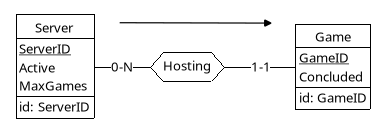
\includegraphics[scale=0.9]{images/Progettazione/Logica/OP2-arrow.png}
\end{figure}

\centerline{\begin{tabular}{ |l|c|c|c| }
\hline
\textbf{Concetto} & \textbf{Costrutto} & \textbf{Accessi} & \textbf{Tipo} \\
\hline
Game & E & 10 & L \\
\hline
Hosting & R & 10 & L \\
\hline
Server & E & 10 & L \\
\hline
& & \textbf{Totale:} 30L $\to$ 10 al giorno & \\
\hline
\end{tabular}}

\subsubsection*{Operazione 3 - Visualizzare tutte le espansioni}
\centerline{\begin{tabular}{ |l|c|c|c| }
\hline
\textbf{Concetto} & \textbf{Costrutto} & \textbf{Accessi} & \textbf{Tipo} \\
\hline
Expansion & E & 4 & L \\
\hline
& & \textbf{Totale:} 4L $\to$ 10 al giorno & \\
\hline
\end{tabular}}

\subsubsection*{Operazione 4 - Creare un nuovo giocatore}
\centerline{\begin{tabular}{ |l|c|c|c| }
\hline
\textbf{Concetto} & \textbf{Costrutto} & \textbf{Accessi} & \textbf{Tipo} \\
\hline
Player & E & 1 & S \\
\hline
& & \textbf{Totale:} 1S $\to$ 40 al giorno & \\
\hline
\end{tabular}}

\subsubsection*{Operazione 5 - Visualizzare tutti i colori}
\centerline{\begin{tabular}{ |l|c|c|c| }
\hline
\textbf{Concetto} & \textbf{Costrutto} & \textbf{Accessi} & \textbf{Tipo} \\
\hline
Color & E & 10 & L \\
\hline
& & \textbf{Totale:} 10L $\to$ 40 al giorno & \\
\hline
\end{tabular}}

\subsubsection*{Operazione 6 - Visualizzare il giocatore corrente}
\centerline{\begin{tabular}{ |l|c|c|c| }
\hline
\textbf{Concetto} & \textbf{Costrutto} & \textbf{Accessi} & \textbf{Tipo} \\
\hline
PlayerInGame & E & 4 & L \\
\hline
& & \textbf{Totale:} 4L $\to$ 700 al giorno & \\
\hline
\end{tabular}}

\subsubsection*{Operazione 7 - Visualizzare la tessera corrente}
\centerline{\begin{tabular}{ |l|c|c|c| }
\hline
\textbf{Concetto} & \textbf{Costrutto} & \textbf{Accessi} & \textbf{Tipo} \\
\hline
Tile & E & 70 & L \\
\hline
& & \textbf{Totale:} 70L $\to$ 700 al giorno & \\
\hline
\end{tabular}}

\subsubsection*{Operazione 8 - Ruotare la tessera corrente}
La rotazione di una tessera prevede che le rispettive sezioni, tranne la centrale, cambino il proprio tipo.
\medskip

\centerline{\begin{tabular}{ |l|c|c|c| }
\hline
\textbf{Concetto} & \textbf{Costrutto} & \textbf{Accessi} & \textbf{Tipo} \\
\hline
Tile & E & 1 & L \\
\hline
Subdivision & R & 12 & L \\
\hline
TileSection & E & 12 & L \\
\hline
Classification & R & 12 & L \\
\hline
Classification & R & 12 & S \\
\hline
TileSectionType & E & 12 & L \\
\hline
& & \textbf{Totale:} 12S + 49L $\to$ 300 al giorno & \\
\hline
\end{tabular}}

\subsubsection*{Operazione 9 - Piazzare la tessera corrente}
Piazzare la tessera corrente porta all'unione con le tessere circostanti, il che implica la modifica dei gameset presenti nelle section. In media sono presenti 2 tile attorno ad una tile appena piazzata, dunque, in media vengono uniti 4 gameset per piazzamento.
\medskip

\centerline{\begin{tabular}{ |l|c|c|c| }
\hline
\textbf{Concetto} & \textbf{Costrutto} & \textbf{Accessi} & \textbf{Tipo} \\
\hline
Tile & E & 1 & L \\
\hline
Tile & E & 1 & S \\
\hline
Subdivision & R & 12 & L \\
\hline
TileSection & E & 12 & L\\
\hline
Location & R & 12 & L \\
\hline
Location & R & 12 & S \\
\hline
Gameset & R & 4 & S \\
\hline
Classification(Gameset) & R & 4 & S \\
\hline
& & \textbf{Totale:} 21S + 37L $\to$ 700 al giorno & \\
\hline
\end{tabular}}

\subsubsection*{Operazione 10 - Piazzare o rimuovere un seguace su una sezione di una tessera}
\centerline{\begin{tabular}{ |l|c|c|c| }
\hline
\textbf{Concetto} & \textbf{Costrutto} & \textbf{Accessi} & \textbf{Tipo} \\
\hline
Meeple & E & 1 & L \\
\hline
Meeple & E & 1 & S \\
\hline
Placement & E & 1 & L \\
\hline
Placement & E & 1 & S \\
\hline
& & \textbf{Totale:} 2S + 2L $\to$ 300 al giorno & \\
\hline
\end{tabular}}

\subsubsection*{Operazione 11 - Visualizzare i seguaci disponibili ad un giocatore}
\centerline{\begin{tabular}{ |l|c|c|c| }
\hline
\textbf{Concetto} & \textbf{Costrutto} & \textbf{Accessi} & \textbf{Tipo} \\
\hline
PlayerInGame & E & 1 & L \\
\hline
Owning & R & 8 & L \\
\hline
Meeple & E & 8 & L \\
\hline
& & \textbf{Totale:} 17L $\to$ 700 al giorno & \\
\hline
\end{tabular}}

\subsubsection*{Operazione 12 - Assegnare un punteggio ad un giocatore}
\centerline{\begin{tabular}{ |l|c|c|c| }
\hline
\textbf{Concetto} & \textbf{Costrutto} & \textbf{Accessi} & \textbf{Tipo} \\
\hline
PlayerInGame & E & 1 & L \\
\hline
PlayerInGame & E & 1 & S \\
\hline
& & \textbf{Totale:} 1S + 1L $\to$ 200 al giorno & \\
\hline
\end{tabular}}

\subsubsection*{Operazione 13 - Aggiornare la tessera corrente}
Aggiornare la tessera corrente implica modificare sia la Tile successiva che la corrente.
\medskip

\centerline{\begin{tabular}{ |l|c|c|c| }
\hline
\textbf{Concetto} & \textbf{Costrutto} & \textbf{Accessi} & \textbf{Tipo} \\
\hline
Tile & E & 2 & L \\
\hline
Tile & E & 2 & S \\
\hline
& & \textbf{Totale:} 2S + 2L $\to$ 700 al giorno & \\
\hline
\end{tabular}}

\subsubsection*{Operazione 14 - Aggiornare il giocatore corrente}
Aggiornare il giocatore corrente implica modificare sia il PlayerInGame successivo che il corrente.
\medskip

\centerline{\begin{tabular}{ |l|c|c|c| }
\hline
\textbf{Concetto} & \textbf{Costrutto} & \textbf{Accessi} & \textbf{Tipo} \\
\hline
PlayerInGame & E & 2 & L \\
\hline
PlayerInGame & E & 2 & S \\
\hline
& & \textbf{Totale:} 2S + 2L $\to$ 700 al giorno & \\
\hline
\end{tabular}}

\subsubsection*{Operazione 15 - Visualizzare le partite non concluse}
\centerline{\begin{tabular}{ |l|c|c|c| }
\hline
\textbf{Concetto} & \textbf{Costrutto} & \textbf{Accessi} & \textbf{Tipo} \\
\hline
Game & E & 10 & L \\
\hline
& & \textbf{Totale:} 10L $\to$ 5 al giorno & \\
\hline
\end{tabular}}

\subsubsection*{Operazione 16 - Visualizzare i giocatori di un partita}
\centerline{\begin{tabular}{ |l|c|c|c| }
\hline
\textbf{Concetto} & \textbf{Costrutto} & \textbf{Accessi} & \textbf{Tipo} \\
\hline
PlayerInGame & E & 4 & L \\
\hline
Participation & R & 4 & L \\
\hline
& & \textbf{Totale:} 8L $\to$ 700 al giorno & \\
\hline
\end{tabular}}

\subsubsection*{Operazione 17 - Visualizzare le tessere piazzate in una partita}
\centerline{\begin{tabular}{ |l|c|c|c| }
\hline
\textbf{Concetto} & \textbf{Costrutto} & \textbf{Accessi} & \textbf{Tipo} \\
\hline
Tile & E & 70 & L \\
\hline
Composition & R & 70 & L \\
\hline
& & \textbf{Totale:} 140L $\to$ 5 al giorno & \\
\hline
\end{tabular}}

\clearpage
\subsubsection*{Operazione 18 - Visualizzare le regioni in ordine di punteggio medio dei giocatori}
\begin{figure}[ht]
    \centering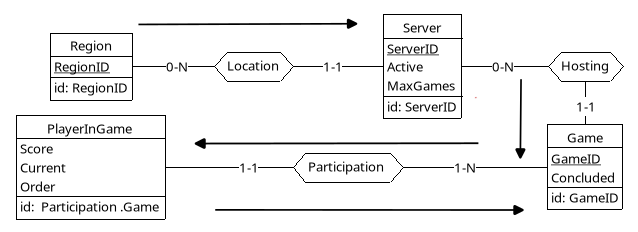
\includegraphics[scale=0.75]{images/Progettazione/Logica/OP18-arrow.png}
\end{figure}

\centerline{\begin{tabular}{ |l|c|c|c| }
\hline
\textbf{Concetto} & \textbf{Costrutto} & \textbf{Accessi} & \textbf{Tipo} \\
\hline
Region & E & 6 & L \\
\hline
Location & R & 10 & L \\
\hline
Server & E & 10 & L \\
\hline
Hosting & R & 10 & L \\
\hline
Game & E & 10 & L \\
\hline
Participation & R & 40 & L \\
\hline
PlayerInGame & E & 40 & L \\
\hline
& & \textbf{Totale:} 126L $\to$ 2 al mese & \\
\hline
\end{tabular}}

\subsubsection*{Operazione 19 - Mostrare per ogni giocatore il numero di avversari con cui ha giocato}
\begin{figure}[ht]
    \centering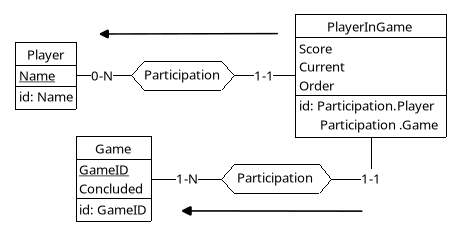
\includegraphics[scale=0.75]{images/Progettazione/Logica/OP19-arrow.png}
\end{figure}

\centerline{\begin{tabular}{ |l|c|c|c| }
\hline
\textbf{Concetto} & \textbf{Costrutto} & \textbf{Accessi} & \textbf{Tipo} \\
\hline
Player & E & 40 & L \\
\hline
Participation(Player) & R & 40 & L \\
\hline
PlayerInGame & R & 40 & L \\
\hline
Participation(Game) & R & 40 & L \\
\hline
& & \textbf{Totale:} 160L $\to$ 4 all'anno & \\
\hline
\end{tabular}}

\subsubsection*{Operazione 20 - Visualizzare per ogni regione l'espansione più giocata}
\begin{figure}[ht]
    \centering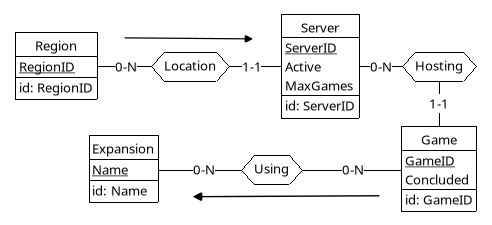
\includegraphics[scale=0.75]{images/Progettazione/Logica/OP20-arrow.png}
\end{figure}
\centerline{\begin{tabular}{ |l|c|c|c| }
\hline
\textbf{Concetto} & \textbf{Costrutto} & \textbf{Accessi} & \textbf{Tipo} \\
\hline
Region & E & 6 & L \\
\hline
Location & R & 10 & L \\
\hline
Server & E & 10 & L \\
\hline
Hosting & R & 10 & L \\
\hline
Game & E & 10 & L \\
\hline
Using & R & 10 & L \\
\hline
Expansion & E & 4 & L \\
\hline
& & \textbf{Totale:} 70L $\to$ 1 al mese & \\
\hline
\end{tabular}}

\subsubsection*{Operazione 21 - Mostrare per ogni colore la probabilità statistica di vincere}
\begin{figure}[ht]
    \centering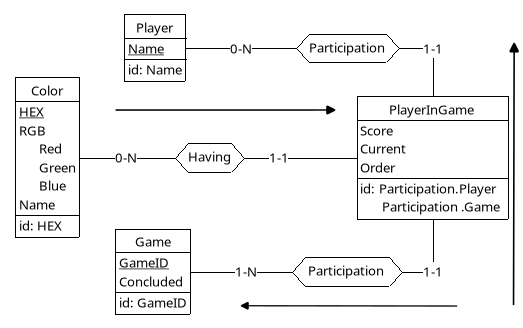
\includegraphics[scale=0.75]{images/Progettazione/Logica/OP21-arrow.png}
\end{figure}
\centerline{\begin{tabular}{ |l|c|c|c| }
\hline
\textbf{Concetto} & \textbf{Costrutto} & \textbf{Accessi} & \textbf{Tipo} \\
\hline
PlayerInGame & E & 40 & L \\
\hline
Participation & R & 40 & L \\
\hline
Game & E & 10 & L \\
\hline
Having & R & 40 & L \\
\hline
Color & E & 10 & L \\
\hline
& & \textbf{Totale:} 140L $\to$ 1 al giorno & \\
\hline
\end{tabular}}

\subsection{Raffinamento dello schema}
\subsubsection*{Eliminazione delle gerarchie}
Per l'eliminazione della gerarchia TileType si è scelto di rimuovere l'entità BasicTile e collassare verso l'alto l'entità ExpansionTile. Questo è stato possibile perché si è deciso di creare un'espansione base contenente tutti i TileType contenuti in BasicTile, rendendo quest'ultima entità inutile. La stessa strategia è stata adottata anche per le gerarchie MeepleType e GamesetType in quanto la situazione era la medesima.

\subsubsection*{Eliminazione degli attributi compositi}
Nello schema l'entità Tile contiene l'attributo composito Position che è stato quindi diviso nelle sue sotto-componenti. Sarà poi compito dell'applicazione accertarsi che tali attributi siano coerenti l'uno con l'altro.

\subsubsection*{Eliminazione degli identificatori esterni}
Nello schema E/R sono state eliminate le seguenti relazioni:
\begin{itemize}
    \item Participation, importando name da players in players\_in\_game
    \item Participation, importando id da games in players\_in\_game
    \item Having, importando hex da colors in players\_in\_game
    \item Owning, importando player\_name e game\_id da players\_in\_game in meeples
    \item Placement, importando name da continents in regions
    \item Specifically, importando name da cardinal\_points in regions
    \item Location, importando id da regions in servers
    \item Hosting, importando id da servers in games
    \item Using, reificata importando id da games e name da expansions
    \item Composition, importando id da games in tiles
    \item Placement, importando id da meeples in tile\_sections
    \item Subdivision, importando game\_id e order da tiles in tile\_sections
    \item Location, importando id da gamesets in tile\_sections
    \item Preceding, importando name da tile\_section\_types in tile\_section\_types
    \item Regarding, importando name da tile\_section\_types in tile\_types\_configurations
    \item Composition, importando name da gameset\_types in tile\_types\_configurations
    \item Description, importando name da tile\_types in tile\_types\_configurations
    \item Classification, importando name da meeple\_types in meeples
    \item Classification, importando name da tile\_section\_types in tile\_sections
    \item Classification, importando name da gameset\_types in gamesets
    \item Classification, importando name da tile\_types in tiles
    \item Using, importando name da expansions in tile\_types
    \item Using, importando name da expansions in gameset\_types
    \item Using, importando name da expansions in meeple\_types
\end{itemize}
In tile\_section\_types abbiamo scelto di importare due volte name da se stessa per avere sia la successiva che la precedente TileSection.

\subsubsection*{Scelta delle chiavi primarie}
La maggior parte delle chiavi primarie sono già evidenziate in modo chiaro nello schema. Da notare l'entità Tile che è identificata tramite l'id della partita e l'ordine preciso in cui viene giocata. Per quanto riguarda l'entità TileSection questa è invece identificata tramite la Tile e il TileSectionType che è univoco all'interno di una Tile. Infine, l'entità TileTypeConfiguration è identificata con il TileType, il TileSectionType e un id aggiuntivo usato per distinguere i vari insiemi di GamesetType uguali presenti sulla Tile di quel TileType. Questo è obbligatorio in quanto su una stessa Tile potrebbero esserci due Gameset da considerare separati con stesso GamesetType.

\subsection{Analisi delle ridondanze}

\subsubsection*{Ridondanza riguardo al campo Placed in Meeple}
Le operazioni 10 e 11 fanno uso del campo Placed in Meeple. Questo costituisce una ridondanza in quanto per verificare se un seguace è stato collocato su una sezione è sufficiente verificare se è presente l'associazione Placement. Nel caso dell'operazione 10, con ridondanza si ha:
\medskip

\centerline{\begin{tabular}{ |l|c|c|c| }
\hline
\textbf{Concetto} & \textbf{Costrutto} & \textbf{Accessi} & \textbf{Tipo} \\
\hline
Meeple & E & 1 & L \\
\hline
Meeple & E & 1 & S \\
\hline
Placement & E & 1 & L \\
\hline
Placement & E & 1 & S \\
\hline
& & \textbf{Totale:} 2S + 2L $\to$ 300 al giorno & \\
\hline
\multicolumn{4}{|l|}{\textbf{Costo Totale} = (2*2 + 2) * 300 = \textbf{1800}} \\
\hline
\end{tabular}}
\medskip

Mentre senza ridondanza si ha:
\medskip

\centerline{\begin{tabular}{ |l|c|c|c| }
\hline
\textbf{Concetto} & \textbf{Costrutto} & \textbf{Accessi} & \textbf{Tipo} \\
\hline
Meeple & E & 1 & L \\
\hline
Placement & E & 1 & L \\
\hline
Placement & E & 1 & S \\
\hline
& & \textbf{Totale:} 2L + 1S $\to$ 300 al giorno & \\
\hline
\multicolumn{4}{|l|}{\textbf{Costo Totale} = (2 + 2) * 300 = \textbf{1200}} \\
\hline
\end{tabular}}
\medskip

Potrebbe quindi sembrare che l'utilizzo della ridondanza sia svantaggioso.
\medskip

Per l'operazione 11 con ridondanza si ottiene:

\centerline{\begin{tabular}{ |l|c|c|c| }
\hline
\textbf{Concetto} & \textbf{Costrutto} & \textbf{Accessi} & \textbf{Tipo} \\
\hline
PlayerInGame & E & 1 & L \\
\hline
Owning & R & 1 & L \\
\hline
Owning & E & 1 & L \\
\hline
& & \textbf{Totale:} 3L $\to$ 700 al giorno & \\
\hline
\multicolumn{4}{|l|}{\textbf{Costo Totale} = 3*700 = \textbf{2100}} \\
\hline
\end{tabular}}
\medskip

Senza la ridondanza:
\medskip

\centerline{\begin{tabular}{ |l|c|c|c| }
\hline
\textbf{Concetto} & \textbf{Costrutto} & \textbf{Accessi} & \textbf{Tipo} \\
\hline
PlayerInGame & E & 1 & L \\
\hline
Owning & R & 1 & L \\
\hline
Meeple & E & 1 & L \\
\hline
Placement & E & 1 & L \\
\hline
& & \textbf{Totale:} 4L $\to$ 700 al giorno & \\
\hline
\multicolumn{4}{|l|}{\textbf{Costo Totale} = 4*700 = \textbf{2800}} \\
\hline
\end{tabular}}
\medskip

Si decide di prediligere l'utilizzo della ridondanza in quanto il costo totale dell'operazione 10 e 11 con ridondanza è minore rispetto a senza.
\medskip

\subsubsection*{Ridondanza riguardo al campo Concluded in Game}
Il campo Concluded, utilizzato nell'operazione 15, è una ridondanza in quanto per dichiarare una partita conclusa è sufficiente verificare se tutte le relative tessere sono state piazzate. Vediamo lo schema con la ridondanza:
\medskip

\centerline{\begin{tabular}{ |l|c|c|c| }
\hline
\textbf{Concetto} & \textbf{Costrutto} & \textbf{Accessi} & \textbf{Tipo} \\
\hline
Game & E & 1 & L \\
\hline
& & \textbf{Totale:} 1L $\to$ 5 al giorno & \\
\hline
\multicolumn{4}{|l|}{\textbf{Costo Totale} = 1*5 = \textbf{5}} \\
\hline
\end{tabular}}
\medskip

Senza ridondanza invece:
\medskip

\centerline{\begin{tabular}{ |l|c|c|c| }
\hline
\textbf{Concetto} & \textbf{Costrutto} & \textbf{Accessi} & \textbf{Tipo} \\
\hline
Game & E & 1 & L \\
\hline
Composition & R & 70 & L \\
\hline
Tile & E & 70 & L \\
\hline
& & \textbf{Totale:} 141L $\to$ 5 al giorno & \\
\hline
\multicolumn{4}{|l|}{\textbf{Costo Totale} = 141*5 = \textbf{705}} \\
\hline
\end{tabular}}

\subsection{Traduzione di entità e associazioni in relazioni}
\hspace{1.5em}players(\textbf{name})\newline

colors(\textbf{hex}, red, green, blue, name)\newline

games(\textbf{id}, server\_id, concluded)\newline
FK: server\_id REFERENCES servers(id)\newline

players\_in\_game(\textbf{player\_name}, \textbf{game\_id}, color\_hex, score, current, order)\newline
FK: player\_name REFERENCES players(name)\newline
FK: game\_id REFERENCES games(id)\newline
FK: color\_hex REFERENCES colors(hex)\newline

games\_expansions(\textbf{expansion\_name}, \textbf{game\_id})\newline
FK: game\_id REFERENCES games(id)\newline
FK: expansion\_name REFERENCES expansions(name)\newline

expansions(\textbf{name})\newline

meeple\_types(\textbf{name}, quantity, strength, expansion\_name)\newline
FK: expansion\_name REFERENCES expansions(name)\newline

meeples(\textbf{id}, owner\_player\_name, owner\_game\_id, type\_name, placed)\newline
FK: owner\_player\_name REFERENCES players\_in\_game(player\_name)\newline
FK: owner\_game\_id REFERENCES players\_in\_game(game\_id)\newline
FK: type\_name REFERENCES meeple\_types(name)\newline

gamesets(\textbf{id}, type\_name, points, closed)\newline
FK: type\_name REFERENCES gameset\_types(name)\newline

gameset\_types(\textbf{name}, starting\_points, endgame\_ratio, expansion\_name)\newline
FK: expansion\_name REFERENCES expansions(name)\newline

tile\_section\_types(\textbf{name}, next\_name*, previous\_name*)\newline
FK: next\_name REFERENCES tile\_section\_types(name)\newline
FK: previous\_name REFERENCES tile\_section\_types(name)\newline

tile\_sections(\textbf{type\_name}, \textbf{tile\_order}, \textbf{tile\_game\_id}, gameset\_id, meeple\_id*, closed)\newline
FK: type\_name REFERENCES tile\_section\_types(name)\newline
FK: tile\_order REFERENCES tiles(order)\newline
FK: tile\_game\_id REFERENCES tiles(game\_id)\newline
FK: meeple\_id REFERENCES meeples(id)\newline
FK: gameset\_id REFERENCES gamesets(id)\newline

tiles(\textbf{order}, \textbf{game\_id}, type\_name, rotation\_count, x\_coordinate*, y\_coordinate*, current)\newline
FK: type\_name REFERENCES tile\_types(name)\newline
FK: game\_id REFERENCES games(id)\newline

tile\_types(\textbf{name}, quantity, expansion\_name)\newline
FK: expansion\_name REFERENCES expansions(name)\newline

tile\_type\_configurations(id, \textbf{tile\_section\_type\_name}, \textbf{tile\_type\_name}, gameset\_type\_name, closed, pennant)\newline
FK: tile\_section\_type\_name REFERENCES tile\_section\_types(name)\newline
FK: tile\_type\_name REFERENCES tile\_types(name)\newline
FK: gameset\_type\_name REFERENCES gameset\_types(name)\newline

regions(\textbf{id}, continent\_name, cardinal\_point\_name*)\newline
FK: continent\_name REFERENCES continents(name)\newline
FK: cardinal\_point\_name REFERENCES cardinal\_points(name)\newline

continents(\textbf{name})\newline

cardinal\_points(\textbf{name})\newline

servers(\textbf{id}, region\_id, active, max\_games)\newline
FK: region\_id REFERENCES regions(id)

\subsection{Schema relazionale finale}
\clearpage
\begin{figure}[ht]
    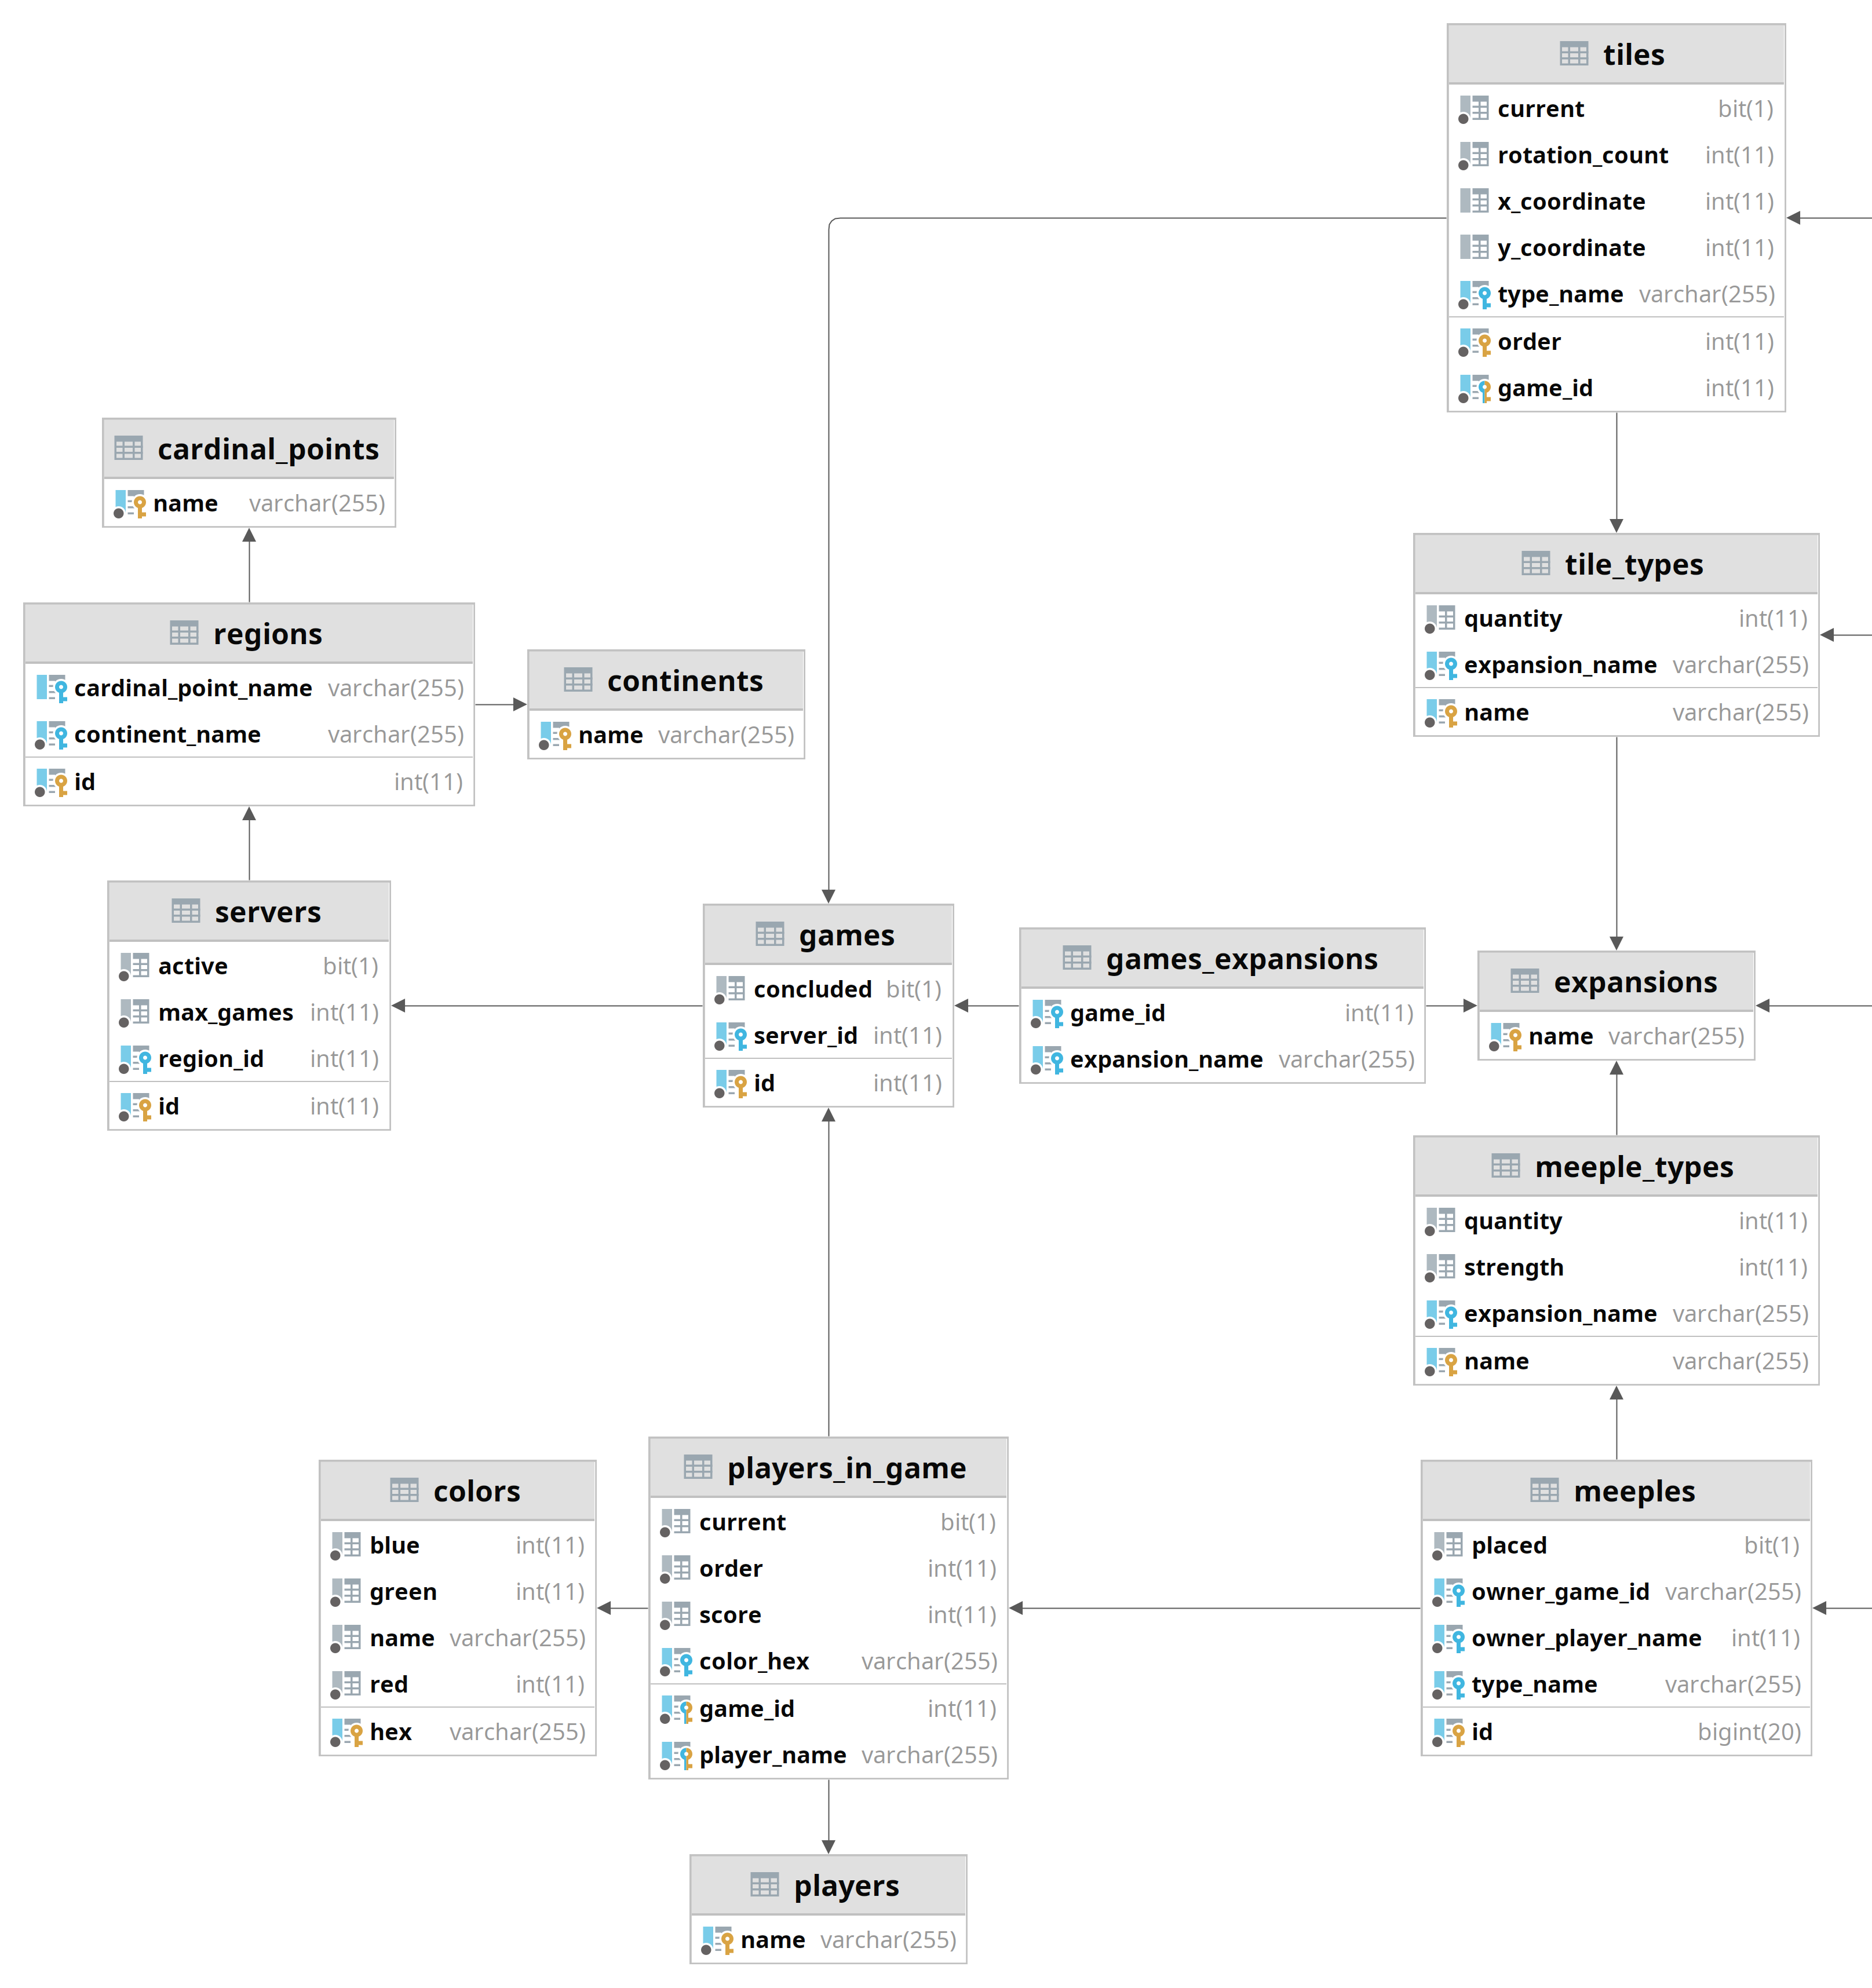
\includegraphics[scale=0.175]{images/Progettazione/relazionale_left.png}
\end{figure}
\clearpage
\begin{figure}[ht]
    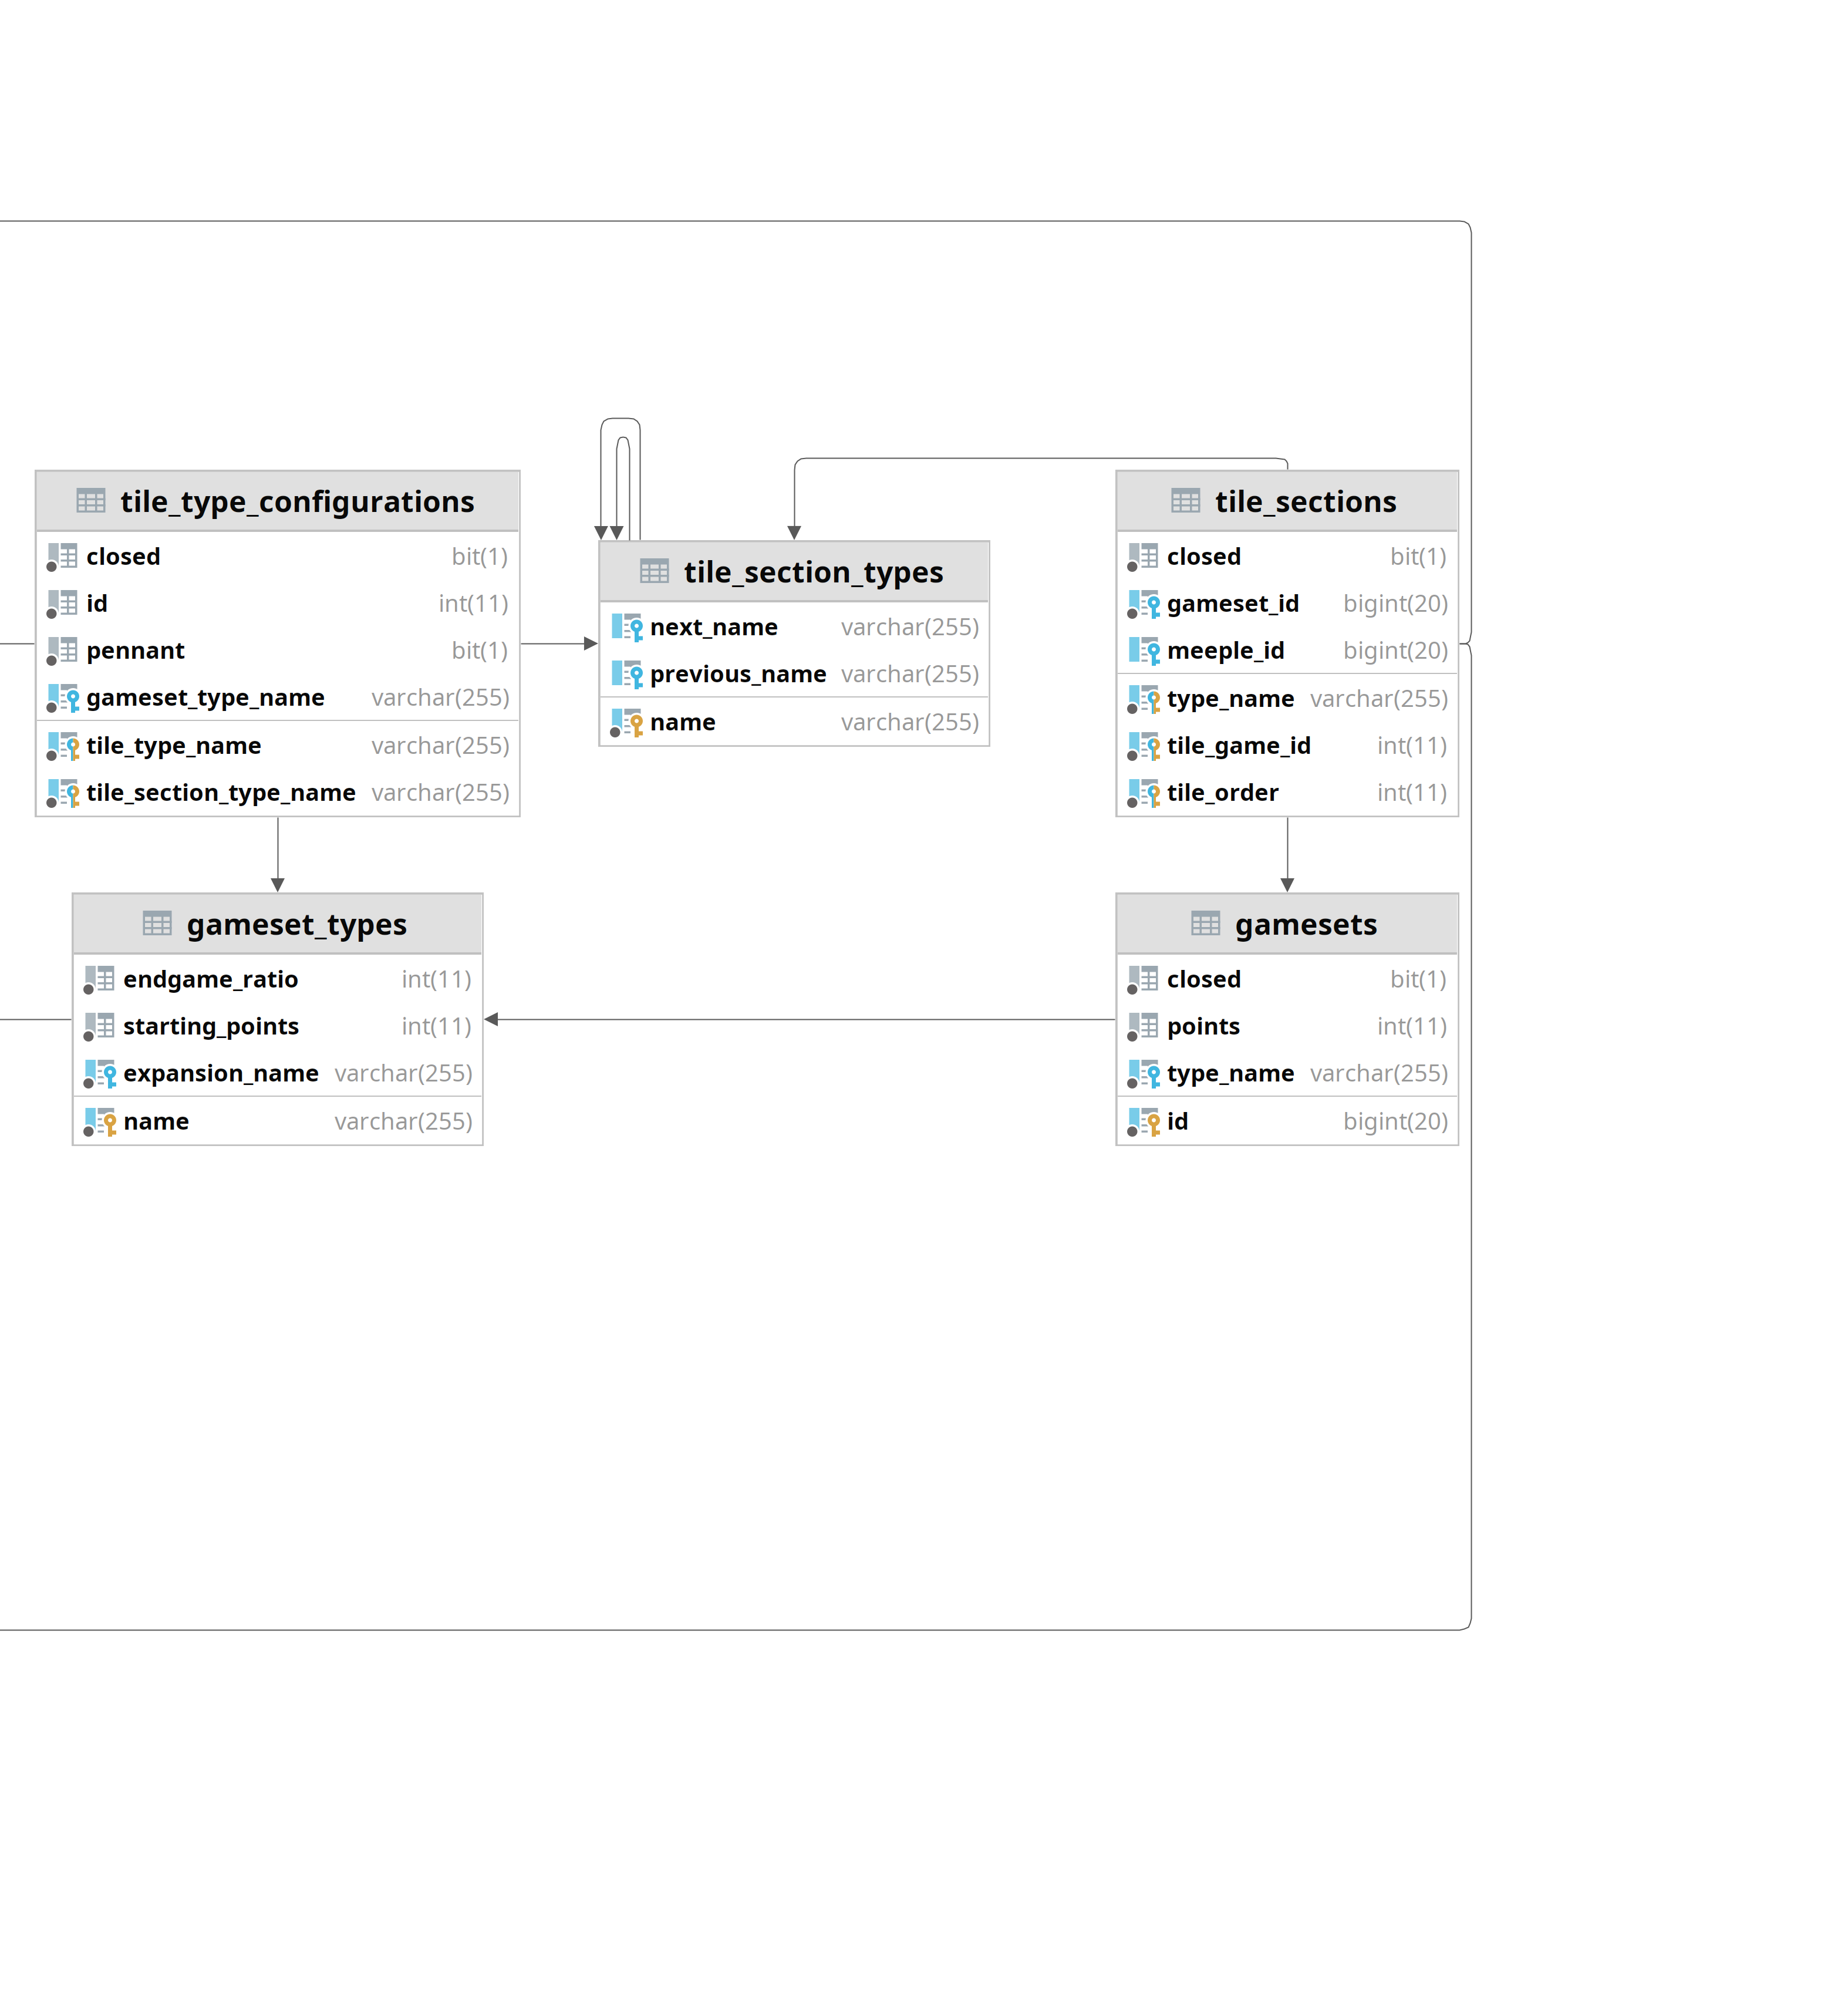
\includegraphics[width=1.247\textwidth, right]{images/Progettazione/relazionale_right.png}
\end{figure}

\clearpage
\subsection{Traduzione delle operazioni in query SQL}
\subsubsection*{OP1 - Creare una nuova partita}
Nel caso in cui i giocatori scelti non esistano nel database vengono creati tramite l'operazione 4. Viene poi creata la partita assieme ai vari players\_in\_game che avranno come game\_id l'id della partita appena creata. Vengono poi creati i seguaci, le strutture e le tessere con le relative sezioni in accordo con le espansioni selezionate alla creazione del gioco.
\medskip

\begin{lstlisting}[style=sql]
    INSERT INTO games (concluded, server_id)
    VALUES (FALSE, ?);

    INSERT INTO players_in_game (current, `order`, score, game_id, player_name, color_hex)
    VALUES (FALSE, ?, 0, ?, ?, ?);

    INSERT INTO meeples (placed, owner_game_id, owner_player_name, type_name)
    VALUES (FALSE, ?, ?, ?);

    INSERT INTO gamesets (closed, points, type_name)
    VALUES (FALSE, 0, ?);

    INSERT INTO tiles (`order`, current, rotation_count, x_coordinate, y_coordinate, game_id, type_name)
    VALUES (?, FALSE, 0, null, null, ?, ?);

    INSERT INTO tile_sections (closed, type_name, tile_game_id, tile_order, gameset_id, meeple_id)
    VALUES (FALSE, ?, ?, ?, ?, null);
\end{lstlisting}

\subsubsection*{OP2 - Visualizzare i server di gioco disponibili}
Un server di gioco è disponibile solo se il numero di partite ancora in corso su quel server è inferiore al suo campo max\_games.
\medskip

\begin{lstlisting}[style=sql]
SELECT *
FROM servers AS s
WHERE active=true AND max_games > (SELECT COUNT(*)
    FROM games AS g
    WHERE g.server_ID=s.ID AND g.concluded = FALSE);
\end{lstlisting}

\subsubsection*{OP3 - Visualizzare tutte le espansioni}
\begin{lstlisting}[style=sql]
    SELECT *
    FROM expansions;
\end{lstlisting}

\subsubsection*{OP4 - Creare un nuovo giocatore}
\begin{lstlisting}[style=sql]
    INSERT INTO players (name)
    VALUES (?);
\end{lstlisting}

\subsubsection*{OP5 - Visualizzare tutti i colori}
\begin{lstlisting}[style=sql]
    SELECT *
    FROM colors;
\end{lstlisting}

\subsubsection*{OP6 - Visualizzare il giocatore corrente}
\begin{lstlisting}[style=sql]
    SELECT *
    FROM players_in_game
    WHERE game_id = ? AND current = TRUE;
\end{lstlisting}

\subsubsection*{OP7 - Visualizzare la tessera corrente}
\begin{lstlisting}[style=sql]
    SELECT *
    FROM tiles
    WHERE game_id = ? AND current = TRUE;
\end{lstlisting}

\subsubsection*{OP8 - Ruotare la tessera corrente}
Per ruotare la tessera corrente bisogna cambiare il tipo delle sezioni ad essa associate, essendo queste parte della chiave si è costretti a rimuoverle per poi re-inserirle aggiornate. Per ogni sezione della tessera corrente bisogna solo aggiornare l'attributo type\_name con il valore dell'attributo next\_name del tipo della sezione in questione, il resto rimane invariato.
\medskip

\begin{lstlisting}[style=sql]
    SELECT *
    FROM tile_sections
    WHERE tile_game_id = ? AND tile_order = ?;

    DELETE
    FROM tile_sections
    WHERE tile_game_id = ? AND tile_order = ?;

    -- Per ogni sezione di tile selezionata con la prima query
    INSERT INTO tile_sections (closed, type_name, tile_game_id, tile_order, gameset_id, meeple_id)
    VALUES (?, ?, ?, ?, ?, ?);
\end{lstlisting}


\subsubsection*{OP9 - Piazzare la tessera corrente}
\begin{lstlisting}[style=sql]
    UPDATE tiles
    SET x_coordinate = ?,
        y_coordinate = ?
    WHERE game_id = ? AND current = TRUE;
\end{lstlisting}

\subsubsection*{OP10 - Piazzare o rimuovere un seguace su una sezione di una tessera}
Nel caso della rimozione di un seguace è invece necessario impostare il relativo attributo placed a false. Inoltre, bisogna anche impostare a null l'attributo meeple\_id della sezione sulla quale era piazzato.
\medskip

\begin{lstlisting}[style=sql]
    UPDATE meeples
    SET placed = TRUE
    WHERE id = ?;

    UPDATE tile_sections
    SET meeple_id = ?
    WHERE type_name = ? AND tile_game_id = ? AND tile_order = ?;
\end{lstlisting}

\subsubsection*{OP11 - Visualizzare i seguaci disponibili ad un giocatore}
Un seguace è disponibile ad un giocatore se non è piazzato.
\medskip

\begin{lstlisting}[style=sql]
    SELECT *
    FROM meeples
    WHERE owner_player_name = ? AND owner_game_id = ? AND placed = FALSE;
\end{lstlisting}

\subsubsection*{OP12 - Assegnare un punteggio ad un giocatore}
\begin{lstlisting}[style=sql]
    UPDATE players_in_game
    SET score = ?
    WHERE game_id = ? AND player_name = ?;
\end{lstlisting}

\subsubsection*{OP13 - Aggiornare la tessera corrente}
Il valore della wildcard per l'attributo order della seconda query si ricava incrementando di 1 l'attributo order della tessera che era prima corrente.
\medskip

\begin{lstlisting}[style=sql]
    UPDATE tiles
    SET current = FALSE
    WHERE game_id = ? AND current = TRUE;

    UPDATE tiles
    SET current = TRUE
    WHERE game_id = ? AND order = ?;
\end{lstlisting}

\subsubsection*{OP14 - Aggiornare il giocatore corrente}
Il valore della wildcard per l'attributo order della seconda query si ricava incrementando di 1 l'attributo order del giocatore che era prima corrente e applicandogli il modulo con il numero di giocatori della partita.
\medskip

\begin{lstlisting}[style=sql]
    UPDATE players_in_game
    SET current = FALSE
    WHERE game_id = ? AND current = TRUE;

    UPDATE players_in_game
    SET current = TRUE
    WHERE game_id = ? AND order = ?;
\end{lstlisting}

\subsubsection*{OP15 - Visualizzare le partire non concluse}
\begin{lstlisting}[style=sql]
    SELECT *
    FROM games
    WHERE concluded = FALSE;
\end{lstlisting}

\subsubsection*{OP16 - Visualizzare i giocatori di una partita}
\begin{lstlisting}[style=sql]
    SELECT *
    FROM players_in_game
    WHERE game_id = ?;
\end{lstlisting}

\subsubsection*{OP17 - Visualizzare le tessere piazzate in una partita}
\begin{lstlisting}[style=sql]
    SELECT *
    FROM tiles
    WHERE game_id = ? AND x_coordinate IS NOT NULL AND y_coordinate IS NOT NULL;
\end{lstlisting}

\subsubsection*{OP18 - Visualizzare le regioni in ordine di punteggio medio dei giocatori}
In questo caso vengono considerate solo le partite concluse.
\medskip

\begin{lstlisting}[style=sql]
SELECT R.id, AVG(P.score) AS AveragePlayerScore
FROM ((regions R INNER JOIN servers S on R.id = S.region_id) INNER JOIN games G ON S.id = G.server_id) INNER JOIN players_in_game P ON G.id = P.game_id
WHERE G.concluded = TRUE
GROUP BY R.id
ORDER BY AveragePlayerScore DESC;
\end{lstlisting}

\subsubsection*{OP19 - Mostrare per ogni giocatore il numero di avversari con cui ha giocato}
Nella subquery per ogni giocatore si conta con quanti altri giocatori diversi e distinti ha giocato.
\medskip

\begin{lstlisting}[style=sql]
SELECT P.player_name, (SELECT COUNT(DISTINCT P2.player_name) AS EnemiesCount
    FROM players_in_game P2 INNER JOIN games G2 on P2.game_id = G2.id
    WHERE G2.id IN (SELECT DISTINCT P3.game_id
        FROM players_in_game P3
        WHERE P3.player_name = P.player_name) AND P2.player_name <> P.player_name) AS EnemiesCount
FROM players_in_game P INNER JOIN games G on P.game_id = G.id
GROUP BY P.player_name
ORDER BY EnemiesCount DESC;
\end{lstlisting}

\subsubsection*{OP20 - Visualizzare per ogni regione l'espansione più giocata}
Per questa operazione si è deciso di non considerare l'espansione base in quanto viene usata in ogni partita. Nella subquery per ogni regione si conta in quante partite è stata usata ogni espansione. Nella query esterna si seleziona solo l'espansione più giocata per ogni regione.
\medskip

\begin{lstlisting}[style=sql]
SELECT SQ.id, SQ.expansion_name, MAX(SQ.GamesCount) AS MaxGamesCount
FROM (SELECT R.id, GE.expansion_name, COUNT(GE.expansion_name) AS GamesCount
    FROM ((regions R INNER JOIN servers S on R.id = S.region_id) INNER JOIN games G ON G.server_id = S.id) INNER JOIN games_expansions GE ON GE.game_id = G.id
    WHERE GE.expansion_name <> 'Basic'
    GROUP BY R.id, GE.expansion_name) AS SQ
GROUP BY SQ.id
ORDER BY SQ.id ASC;
\end{lstlisting}

\subsubsection*{OP21 - Mostrare per ogni colore la probabilità statistica di vincere}
Viene effettutata una subquery per ricavare i vincitori delle partite e in questo modo tramite un raggruppamento e una somma viene individuato il numero di vincitori per ogni colore. Viene infine effettutata una divisione tra il numero dei vincitori e il totale delle tuple così da ottenere la probabilità di vincere sulla base del colore scelto.
\medskip

\begin{lstlisting}[style=sql]
SELECT c.name, (SUM(CASE WHEN pig.Score = max_scores.max_score THEN 1 ELSE 0 END) / COUNT(*)) AS WinProbability
FROM colors c JOIN players_in_game pig ON c.hex = pig.color_hex JOIN (SELECT game_id, MAX(Score) AS max_score
FROM players_in_game
GROUP BY game_id) max_scores ON pig.game_id = max_scores.game_id JOIN games g ON pig.game_id = g.id
WHERE g.concluded = TRUE
GROUP BY c.hex, c.name;
\end{lstlisting}
